\chapter{Keys and Addresses}
\label{ch:keys-and-addresses}

\begin{summary}
In this chapter we introduce Bitcoin’s keys and addresses and describe how they are created and the rationale behind that process. We then go through different wallet types and how these keys can be used in practice.
\end{summary}

\section{Private Keys}
Bitcoin uses the Elliptic Curve Digital Signature Algorithm (ECDSA)\footnote{https://en.wikipedia.org/wiki/Elliptic\_Curve\_Digital\_Signature\_Algorithm} to create its private-public key pairs. The exact elliptic curve parameters used in Bitcoin are defined by secp256k1\footnote{https://en.bitcoin.it/wiki/Secp256k1}.

\begin{note}
In ECDSA a private key can be used to calculate the corresponding public key, and since a Bitcoin address is calculated from the public key, if you hold a private key securely you effectively have everything.
\end{note}

The ECDSA private key in Bitcoin is just a very large random number consisting of 256 bits or 32 bytes or 64 hexadecimal digits. Nearly all 256-bit numbers can be valid private keys as specified in secp256k1.

To display a private key (the bytes) we need to format it appropriately. It could be displayed in hex but the most common format used to display a private key is Wallet Import Format (WIF) or WIF-compressed (WIFC); both are a Base58Check\footnote{https://en.bitcoin.it/wiki/Base58Check\_encoding} encoding of the ECDSA key; Base58\footnote{https://en.wikipedia.org/wiki/Base58} with a version prefix to specify the network and a 32-bit checksum.

A WIF-compressed adds an extra byte (0x01) at the end of the ECDSA key before the Base58Check encoding. It specifies whether the public key (and by extension addresses) will be compressed or not. By default most wallets use WIFC format in order to reduce the size of the blockchain\footnote{Note that the segregated witness upgrade allows only compressed public keys.}.


\begin{note}
The WIFC will be 33 bytes long. The compression is happening when creating the public key which will be 33 bytes instead of 65 bytes.
\end{note}

The following is pseudocode of the process that converts the private key to WIF.

\begin{emphbox}
%\begin{lstlisting}[style=Pseudomath,label={lst:wif-pseudocode},caption={Pseudocode to convert a private key to the WIF format},captionpos=b]
\begin{lstlisting}
key_bytes = (32 bytes number) [ + 0x01 if compressed ]
network_prefix = (1 byte version number)
data = network_prefix + key_bytes
data_hash = SHA-256( SHA-256( data ) )
checksum = (first 4 bytes of data_hash)
wif = Base58CheckEncode( data + checksum )
\end{lstlisting}
\end{emphbox}

Note that all the above functions operate on big-endian bytes. The network prefix specifies the Bitcoin network that this private key would be used\footnote{The same private key can be of course used in both mainnet and testnet or even other compatible cryptocurrencies by using the appropriate prefix when generatig the WIF.}. The Base58 WIF prefix depends on the network prefix and whether it is compressed or not, as shown in table~\ref{tab:private-key-prefixes}.

\begin{table}[h]
\centering
\begin{tabular}{ |l|c|c|c|c| }
\hline
~ & \multicolumn{2}{c|}{\textbf{Mainnet}} & \multicolumn{2}{c|}{\textbf{Testnet}} \\
\hline
ECDSA HEX & \multicolumn{2}{c|}{64 digits number} & \multicolumn{2}{c|}{64 digits number} \\
\hline
ECDSA HEX-C & \multicolumn{2}{c|}{Above number + ``01''} & \multicolumn{2}{c|}{Above number + ``01''} \\
\hline
~ & \textbf{Network Prefix} & \textbf{Base58 Prefix} & \textbf{Network Prefix} & \textbf{Base58 Prefix} \\
\hline
WIF & 128 | 0x80 & 5 & 239 | 0xef & 9 \\
\hline
WIF-C & 128 | 0x80 & K or L & 239 | 0xef & c \\
\hline
\end{tabular}
\caption{Private keys network prefixes}
\label{tab:private-key-prefixes}
\end{table}

As an example let us use the following hexadecimal number\footnote{In decimal: 6273083586486421860511804118443655246000698298582245067579657211. It is important to understand that a random number with enough entropy is required for your private key to be secure. A number representing your date of birth or your name’s characters, etc. will be found immediately by software and you will lose your funds.}:

\begin{emphbox}
0dde70823a4bb0ca3bd75a2010e8d5dc091185e73d8b4257a981c695a3eba95b
\end{emphbox}

You can now consult table~\ref{tab:private-key-example} for its compressed version and the corresponding WIF and WIF-C.

\begin{table}[h]
\centering
\begin{tabular}{ |l|l| }
\hline
HEX & 0dde70823a4bb0ca3bd75a2010e8d5dc091185e73d8b4257a981c695a3eba95b \\
\hline
HEX-C & 0dde70823a4bb0ca3bd75a2010e8d5dc091185e73d8b4257a981c695a3eba95b\textbf{01} \\
\hline
WIF & 91h2ReUJRwJhTNd828zhc8RRVMU4krX9q3LNi4nVfiVwkMPfA9p \\
\hline
WIF-C & cN3fHnPVw4h7ZQSRz2HgE3ko69LTaZa5y3JWpFhoXtAke4MiqVQo \\
\hline
\end{tabular}
\caption{Private key network prefix examples}
\label{tab:private-key-example}
\end{table}

Let's use the bitcoin-utils library to construct the WIF and WIFC.

\vspace{1em}
\begin{lstlisting}[style=Python,label={lst:construct-wif},caption={Example of creating WIF and WIFC using Python},captionpos=b]
>>> from bitcoinutils.setup import setup
>>> from bitcoinutils.keys import PrivateKey
>>> setup('testnet')                                   # use testnet parameters
'testnet'
>>> secret_exponent = 0x0dde70823a4bb0ca3bd75a2010e8d5dc091185e73d8b4257a981c695a3eba95b
>>> priv = PrivateKey(secret_exponent = secret_exponent)
>>> priv.to_wif(compressed=False)
'91h2ReUJRwJhTNd828zhc8RRVMU4krX9q3LNi4nVfiVwkMPfA9p'
>>> priv.to_wif(compressed=True)                       # the default
'cN3fHnPVw4h7ZQSRz2HgE3ko69LTaZa5y3JWpFhoXtAke4MiqVQo'
\end{lstlisting}
\vspace{1em}

The actual Python implementation of the functionality demonstrated above can be found at \keyword{to\_wif()}\footnote{\url{https://github.com/karask/python-bitcoin-utils/blob/42875a3fa90d267f2e5e17e017cb28fc8a90c5a8/bitcoinutils/keys.py\#L169-L193}} on github. You can also check how we can get to the private key bytes from WIF in \keyword{\_from\_wif()}\footnote{\url{https://github.com/karask/python-bitcoin-utils/blob/42875a3fa90d267f2e5e17e017cb28fc8a90c5a8/bitcoinutils/keys.py\#L129-L166}}. Feel free to consult the rest of the code and/or the examples in the repository.

Another tool that you can use from the command line is BX\footnote{https://github.com/libbitcoin/libbitcoin-explorer/wiki/Download-BX}. It has extensive capabilities including creating WIFs.

\begin{emphbox}
\begin{lstlisting}[style=Bash]
$ ./bx base58check-encode --version 239 \\
0dde70823a4bb0ca3bd75a2010e8d5dc091185e73d8b4257a981c695a3eba95b
91h2ReUJRwJhTNd828zhc8RRVMU4krX9q3LNi4nVfiVwkMPfA9p

$ ./bx base58check-encode --version 239 \\
0dde70823a4bb0ca3bd75a2010e8d5dc091185e73d8b4257a981c695a3eba95b01
cN3fHnPVw4h7ZQSRz2HgE3ko69LTaZa5y3JWpFhoXtAke4MiqVQo
\end{lstlisting}
\end{emphbox}


\section{Public Keys}
In ECDSA a public key is generated from the private key. Elliptic curves operate over finite fields\footnote{https://en.wikipedia.org/wiki/Finite\_field} and thus all points on the curve are limited to integer coordinates; a finite field is typically accomplished by applying modulo p, where p is a prime number. The specific curve that Bitcoin uses (secp256k1) is  $y^2 = x^3 + 7$ (see figure~\ref{fig:ecdsa-curve}\footnote{From https://cryptobook.nakov.com/asymmetric-key-ciphers/elliptic-curve-cryptography-ecc}). Then the public key P is generated by multiplying, using elliptic curve multiplication, the private key k with a special constant G called the generator point\footnote{This is a special point in the elliptic curve that is pre-defined in secp256k1.}: $P = k * G$. Elliptic curve multiplication of an integer with a point results in another point in the curve, which is the public key.

\begin{figure}[h]
\begin{center}
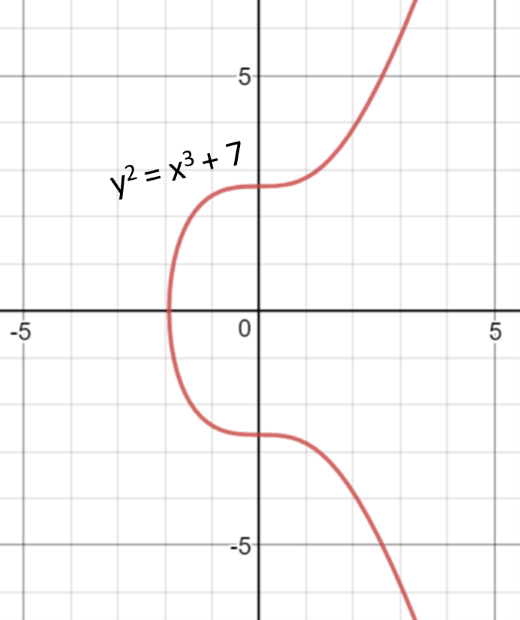
\includegraphics[scale=0.5]{images/ecdsa-curve}
\caption{The secp256k1 ECDSA curve.}
\label{fig:ecdsa-curve}
\end{center}
\end{figure}

The public key is a point $P$ in the elliptic curve. $P = (x,y)$, where both $x$ and $y$ are 32-byte integers. Thus a public key can be expressed with 64 bytes. In Bitcoin, we encode a public key by a prefix that specifies some extra information.

\begin{note}
Remember that we can represent a public key in two forms, compressed and uncompressed. This is where we can reduce the size of the blockchain by using the compressed form.
\end{note}

An encoded uncompressed public key is 65 bytes long since it has the two points (32 bytes each) concatenated and a prefix of \keyword{0x04} to specify an uncompressed public key.

Since the curve is mirrored in the x axis the y coordinate can only take 2 values for a specific x (positive/negative). Thus, an encoded compressed public key is only 33 bytes long and has only the x coordinate with a prefix of \keyword{0x02} (when y is positive/even) or \keyword{0x03} (when y is negative/odd).

Let's use the bitcoin-utils library to construct a private key object from a WIF and use that to create a public key object to show its two forms.

\vspace{1em}
\begin{lstlisting}[style=Python,label={lst:display-public-keys},caption={Python example to generate compressed and uncompressed public keys},captionpos=b]
>>> from bitcoinutils.setup import setup
>>> from bitcoinutils.keys import PrivateKey, PublicKey
>>> setup('testnet')
'testnet'
>>> priv = PrivateKey.from_wif('91h2ReUJRwJhTNd828zhc8RRVMU4krX9q3LNi4nVfiVwkMPfA9p')
>>> pub = priv.get_public_key()
>>> pub.to_hex()                # default is compressed form
'02c1acdac799fb0308b4b6475ddf7967676759d31484ab55555482472f3bc7c3e7'
>>> pub.to_hex(compressed=False)
'04c1acdac799fb0308b4b6475ddf7967676759d31484ab55555482472f3bc7c3e7\\
addc4cbba6656a4be4bc6933a6af712b897a543a09c4b899e5f7b943d38108a8'
\end{lstlisting}
\vspace{1em}

You can see in lines 10-11 in listing~\ref{lst:display-public-keys} that the uncompressed public key has the same $x$ coordinate as the compressed one plus the $y$ coordinate.

To create the PublicKey from the PrivateKey object we make use\footnote{It is always recommended to reuse well-tested cryptography libraries than implementing your own.} of the python ecdsa library as can be seen in \keyword{get\_public\_key()} on github\footnote{\url{https://github.com/karask/python-bitcoin-utils/blob/fb0849f81117943563b17f1870a9607d48ca9653/bitcoinutils/keys.py\#L351-L355}}. The PublicKey object holds the $x$ and $y$ coordinates and can convert accordingly. It checks if $y$ is even or odd and prefixes it with $0x02$ and $0x03$ respectively. You can check the code of \keyword{to\_hex()} on github\footnote{\url{https://github.com/karask/python-bitcoin-utils/blob/fb0849f81117943563b17f1870a9607d48ca9653/bitcoinutils/keys.py\#L453-L469}}.

We can get the public keys from the private keys using BX again.

\begin{emphbox}
\begin{lstlisting}[style=Bash]
$ ./bx wif-to-public 91h2ReUJRwJhTNd828zhc8RRVMU4krX9q3LNi4nVfiVwkMPfA9p
04c1acdac799fb0308b4b6475ddf7967676759d31484ab55555482472f3bc7c3e7\\
addc4cbba6656a4be4bc6933a6af712b897a543a09c4b899e5f7b943d38108a8

$ ./bx wif-to-public cN3fHnPVw4h7ZQSRz2HgE3ko69LTaZa5y3JWpFhoXtAke4MiqVQo
02c1acdac799fb0308b4b6475ddf7967676759d31484ab55555482472f3bc7c3e7
\end{lstlisting}
\end{emphbox}


\section{Addresses}
\label{sec:addresses}
Addresses can be shared to anyone who wants to sent you money. They are typically generated from the public key, consist of a sequence of characters and digits and start with 1 for the mainnet and with m or n for testnet\footnote{Or for segwit addresses bc1 and tb1 for mainnet and testnet respectively.}.

An address typically represents the owner of a private/public pair but it can also represent a more complex script as we will see in a future chapter.

Notice that we do not share the public key as one would expect in public key cryptography but rather the address, which is derived from the public key. Some benefits are:

\begin{itemize}
\item shorter addresses
\item quantum computer resistance
\end{itemize}

\begin{note}
Until one spends from an address the public key will never appear on the blockchain and thus to potential attackers and since the address is hashed from the public key not even quantum computers could brute force to get the public key and then the private key. Note, however, that even if that is the case the majority of addresses would be hacked thus destroying trust in (and the value of) the network anyway!
\end{note}

\subsection*{Legacy Addresses}
\label{ssec:legacy-addresses}

An address is really just the hash of the public key, called public key hash (or PKH). That is how it is represented on the blockchain. The way we format addresses to display them (starting with 1, m/n, etc.) are just for our convenience. The format that we use is the Base58Check encoding of the public key hash; Base58 with version prefix to specify the network and a 32-bit checksum.

The following is pseudocode of the process that converts the public key to public key hash and then address:

\begin{emphbox}
%\begin{lstlisting}[style=Pseudomath,label={lst:address-pseudocode},caption={Pseudocode to convert a public key to an address},captionpos=b]
\begin{lstlisting}
network_prefix = (1 byte version number)
keyHash = RIPEMD-160( SHA-256( publicKey ) )
data = network_prefix + keyHash
dataHash = SHA-256( SHA-256( data ) )
checksum = (first 4 bytes of dataHash)
address = Base58CheckEncode( data + checksum )
\end{lstlisting}
\end{emphbox}

Note that all the above functions operate on big-endian bytes. The network prefix specifies the Bitcoin network that this private key would be used. The Base58 WIF prefix depends on the network prefix and whether it is compressed or not, as shown in table~\ref{tab:address-prefixes}.

\begin{table}[h]
\centering
\begin{tabular}{ |l|c|c|c|c| }
\hline
~ & \multicolumn{2}{c|}{\textbf{Mainnet}} & \multicolumn{2}{c|}{\textbf{Testnet}} \\
\hline
~ & \textbf{Network Prefix} & \textbf{Base58 Prefix} & \textbf{Network Prefix} & \textbf{Base58 Prefix} \\
\hline
P2PKH & 0 | 0x00 & 1 & 111 | 0x6f & m or n \\
\hline
P2SH & 5 | 0x05 & 3 & 196 | 0xc4 & 2 \\
\hline
\end{tabular}
\caption{Addresses network prefixes}
\label{tab:address-prefixes}
\end{table}

\keyword{P2PKH} stands for Pay to Public Key Hash and is the typical legacy address. \keyword{P2SH} stands for Pay to Script Hash and is the typical legacy script hash address; an address that is protected with an arbitrary script rather than just a private-public key pair as in the P2PKH case.

Let's use the bitcoin-utils library to construct some addresses; compressed and uncompressed.

\vspace{1em}
\begin{lstlisting}[style=Python,label={lst:display-addresses},caption={Python example to generate compressed and uncompressed addresses},captionpos=b]
>>> from bitcoinutils.setup import setup
>>> from bitcoinutils.keys import PrivateKey, PublicKey, P2pkhAddress
>>> setup('testnet')
'testnet' 
>>> priv = PrivateKey.from_wif('91h2ReUJRwJhTNd828zhc8RRVMU4krX9q3LNi4nVfiVwkMPfA9p')
>>> pub = priv.get_public_key()  
>>> addr1 = pub.get_address()
>>> addr2 = pub.get_address(compressed=False)
>>> addr1.to_string()
'n42m3hGC52QTChUbXq3QAPVU6nWkG9xuWj' 
>>> addr2.to_string() 
'n2JjAgC6UqFf8DvsZXhWcyNzm8w8YKj7MQ'
\end{lstlisting}
\vspace{1em}

\begin{note}
Since the hash of a compressed public key would be different from the hash of an uncompressed public key we have two distinct legacy addresses.
\end{note}

The actual python implepmentation of converting a public key hash (the application of SHA256 and then RIPEMD160, also called HASH160) can be found at \keyword{\_to\_hash160()} on github\footnote{\url{https://github.com/karask/python-bitcoin-utils/blob/52b7d906f2db8ec4ed4945a04b7e4da2d1db369c/bitcoinutils/keys.py\#L589-L597}}. For code to convert from public key hash to address consult \keyword{to\_string()}\footnote{\url{https://github.com/karask/python-bitcoin-utils/blob/52b7d906f2db8ec4ed4945a04b7e4da2d1db369c/bitcoinutils/keys.py\#L802-L824}}. Feel free to consult the rest of the code and/or the examples in the repository for segwit address creation, etc.


\subsection*{Native Segregated Witness Addresses}

Segregated Witness (segwit) is a consensus change that was activated in August 2017 and introduces an update on how transactions are constructed. It introduces two new transaction types, Pay-to-Witness-Public-Key-Hash (P2WPKH) and Pay-to-Witness-Script-Hash (P2WSH). These new transaction types are going to be explained in section \ref{sec:segwit}.

Native segwit addresses use a different format to display the public key hash called Bech32 encoding\footnote{https://github.com/bitcoin/bips/blob/master/bip-0173.mediawiki} (instead of Base58check). For code implementation look at the python reference implementation\footnote{\url{https://github.com/karask/python-bitcoin-utils/blob/52b7d906f2db8ec4ed4945a04b7e4da2d1db369c/bitcoinutils/bech32.py}} by Pieter Wuille.

The network prefix specifies the Bitcoin network that this address would be used. Specifically, mainnet addresses start with \keyword{bc1}, testnet with \keyword{tb1} and regtest\footnote{Legacy addresses use the same prefix as testnet.} with \keyword{bcrt1}. The size of the address differentiates between public key hashes and script hashes; P2WPKH are 20 bytes long and P2WSH are 32 bytes long.

Let's use the bitcoin-utils library to construct a segwit address.

\vspace{1em}
\begin{lstlisting}[style=Python,label={lst:display-segwit-address},caption={Example of displaying a segwit address from a public key using Python},captionpos=b]
>>> from bitcoinutils.setup import setup
>>> from bitcoinutils.keys import PrivateKey, PublicKey, P2wpkhAddress
>>> setup('testnet')
'testnet' 
>>> priv = PrivateKey.from_wif('91h2ReUJRwJhTNd828zhc8RRVMU4krX9q3LNi4nVfiVwkMPfA9p')
>>> pub = priv.get_public_key()  
>>> addr = pub.get_segwit_address()
>>> addr.to_string() 
'tb1q7m6ak6k050sxzxjjekhey73k0f3rqnxsqa08k2'
\end{lstlisting}
\vspace{1em}



\subsection*{Nested Segregated Witness Addresses}

When segwit was introduced a lot of wallets did not support the new bech32 addresses, so users could not use them to send funds to segwit addresses. To remedy that, nested segwit addresses could be used.

Effectively you could nest or wrap a segwit address into a P2SH address. As already mentioned P2SH addresses can be created from arbitrary scripts and thus could also include a witness script. Again, P2SH and segwit are outside our scope for now and will be explained in more detail in section \ref{sec:segwit}.

\begin{note}
	After the segwit upgrade one needs to choose the type of address to create (e.g. when using \keyword{getnewaddress}). The supported types where \keyword{legacy}, \keyword{p2sh-segwit} and \keyword{bech32}. The default, starting from version 0.16.0, was nested segwit addresses (\keyword{p2sh-segwit}) and from version 0.19 onwards the default is segwit addresses (\keyword{bech32}). The default can be changed in the configuration using \keyword{addresstype}.
\end{note}


\subsection*{Vanity Addresses}
These are normal addresses that contain a specific string. They are calculated randomly by creating random private keys and then checking if the corresponding address starts with that string, e.g. \keyword{1KK}.

\vspace{1em}
\begin{lstlisting}[style=Python,label={lst:vanity-address-example},caption={Example of creating a vanity address using Python},captionpos=b]
import random
from bitcoinutils.setup import setup
from bitcoinutils.keys import PrivateKey

setup('mainnet')

vanity_string = '1KK'
found = False
attempts = 0

while(not found):
    p = PrivateKey(secret_exponent = random.getrandbits(256))
    a = p.get_public_key().get_address()
    print('.', end='', flush=True)
    attempts += 1
    if(a.to_string().startswith(vanity_string)):
        found = True

print("\nAttempts: {}".format(attempts))
print("Address: {}".format(a.to_string()))
print("Secret Key: {}".format(p.to_wif()))
\end{lstlisting}
\vspace{1em}

You will notice that it takes some time even for a short string. Legacy addresses always start with 1 so we can disregard that. Since addresses use base58 each character will take an average of $58$ attempts to be found. The next character an additional $58$ attempts (thus $58*58$). We can generalize with $58^{n}$ where $n$ is the number of characters the vanity address should start with. 

There are efficient implementations for calculating vanity addresses in C, Go, Rust or other compiled system languages that will calculate much faster than our simple example above, but still to create a vanity address that starts with \keyword{1Kostas} will require 38,068,692,544 attempts ($58^{6}$). That will take considerable time regardless of the efficiency of the program or the hardware used.

In practice, these large vanity addresses are created via \emph{vanity address pools}. Such pools have specialized hardware (i.e. mining hardware) that can create vanity addresses fast, albeit for a fee. However, how can they send you your private key that corresponds to the vanity address without them knowing it?

\subsubsection*{Vanity Address Pools}
Vanity address pools take advantage of an elliptic curve arithmetics property in which the public key of the sum of two public keys corresponds to the private key of the sum of the corresponding public keys. For example consider Alice having the key pair a-A and Bob the key pair b-B, then:

\begin{emphbox}
\begin{lstlisting}[style=Pseudomath]
A+B will produce the public key of the a+b private key.
\end{lstlisting}
\end{emphbox}

Consider that Alice wants to use a pool operated by Bob to get a vanity address. Figure~\ref{fig:vanity-address-pools} illustrates the process to securely get to the private key that corresponds to the vanity address.

\begin{figure}[h]
\begin{center}
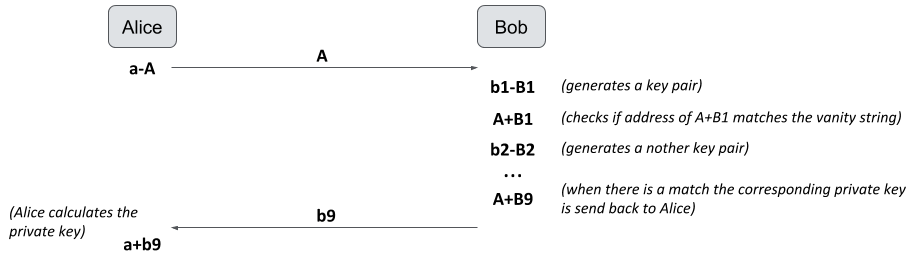
\includegraphics[scale=0.5]{images/vanity-address-pools}
\caption{Example of how a vanity address pool securely shares the private key to a user.}
\label{fig:vanity-address-pools}
\end{center}
\end{figure}

\begin{itemize}
\item First Alice creates a key pair and sends the public key \keyword{A} to Bob.
\item Bob creates a key pair and adds the new public key \keyword{B1} to Alice's key. Then uses the resulting public key to generate an address. If this address does not match the vanity string required by Alice, it repeats the process by creating another key pair, and so on. When a match is found the respective private key, e.g. \keyword{b9}, is send to Alice.
\item Now Alice, and only Alice, can construct a private key that corresponds to the vanity address by adding it to her private key. 
\end{itemize}



\section{Wallets}

A wallet is software that allows us to manage the private and public keys as well as our Bitcoin addresses. They usually have functionality to send bitcoins, check balances, create contact lists and other. Usually a key (i.e. address) is used only once. Depending on how the private keys are handled there are two types of wallets:

\begin{description}
\item[Non-deterministic] All the private keys on the wallet are just randomly generated. Several private keys are pre-generated and new keys are created if needed. If you backup your wallet and then create new keys, you will need to backup your wallet again.
\item[Deterministic] A seed is used to create a master private key, which can be used to create all other private keys (thus public keys and addresses as well). If you backup your seed you are safe no matter how many keys you use since all can be generated from the seed.
\end{description}

Nowadays, most wallets are \emph{Hierarchical Deterministic (HD)} since they offer more flexibility, easier backups and enchanced security in certain use cases. HD wallets are described in detail in \emph{Bitcoin Improvement Proposals (BIPs)} 32\footnote{https://github.com/bitcoin/bips/blob/master/bip-0032.mediawiki}, 43\footnote{https://github.com/bitcoin/bips/blob/master/bip-0043.mediawiki} and 44\footnote{https://github.com/bitcoin/bips/blob/master/bip-0044.mediawiki}. 


\section{More examples}
This section will provide more examples of how to create and use keys and addresses using the \keyword{bitcoin-utils} Python library.

\subsection*{Create a P2SH-P2WPKH address}
In this example we will create and display a P2SH address that wraps a P2WPKH script. For more details on what P2SH and P2WPKH are please refer to sections \ref{sec:p2sh} and \ref{sec:segwit} respectively.

\vspace{1em}
\begin{lstlisting}[style=Python]
>>> from bitcoinutils.setup import setup
>>> from bitcoinutils.keys import PrivateKey, P2shAddress 
>>> setup('testnet')
'testnet'
>>> native_p2wpkh = PrivateKey.from_wif('cTmyBsxMQ3vyh4J3jCKYn2A'\
...         'u7AhTKvqeYuxxkinsg6Rz3BBPrYKK').get_public_key().get_segwit_address()
>>> print("P2WPKH:", native_p2wpkh.to_string())
P2WPKH: tb1qsd4ax84vhem5hxgxus2u232nw9ylgftkz0szf2
>>> nested_p2wpkh = P2shAddress.from_script(native_p2wpkh.to_script_pub_key())
>>> print("P2SH(P2WPKH):", nested_p2wpkh.to_string())
P2SH(P2WPKH): 2N8Z5t3GyPW1hSAEJZqQ1GUkZ9ofoGhgKPf
\end{lstlisting}
\vspace{1em}


\subsection*{Sign message with private key and verify}
We can use a private key to sign a message. In asymmetric cryptography, the recipient can then use the corresponding public key to verify that the message was not tampered with.

\vspace{1em}
\begin{lstlisting}[style=Python,label={lst:sign-verify-message},caption={Use public key to sign a message and them verify},captionpos=b]
>>> from bitcoinutils.setup import setup
>>> from bitcoinutils.keys import P2pkhAddress, PrivateKey, PublicKey
>>> setup('testnet')
'testnet'
>>> priv = PrivateKey.from_wif('91h2ReUJRwJhTNd828zhc8RRVMU4krX9q3LNi4nVfiVwkMPfA9p')
>>> address = priv.get_public_key().get_address()
>>> message = "The test!"
>>> signature = priv.sign_message(message)
>>> print("The signature is:", signature)
The signature is: INzSwXNYNUkPFImslSFDzvqoib3ZdODcaBSZHvx5e4z1wc64cF1dVMZbDFtZxYBlD\\
L/dsjK2iBD5qAf7VcmSdQo=
>>> if PublicKey.verify_message(address.to_string(), signature, message):
...     print("The signature is valid!")
... else:
...     print("The signature is NOT valid!")
...
The signature is valid!
\end{lstlisting}
\vspace{1em}

\begin{note}
We verify using the address instead of the public key. In ECDSA cryptography the public key can be reconstructed given the signature and the public key hash (or address).
\end{note}


\section{Exercises}

\begin{exercise}
Describe possible outcomes of mistyping a Bitcoin address when trying to send some bitcoins.
\end{exercise}

\begin{exercise}
Use a \emph{vanity generator}, like https://github.com/samr7/vanitygen, to create some addresses.
\end{exercise}

\begin{exercise}
Use Python and the \keyword{bitcoin-utils} library to create a simple vanity generator.
\end{exercise}

\begin{exercise}
Write a function that creates a Bitcoin address given a public key. The only Python libraries that you are allowed to use are \keyword{hashlib} for the hashing algorithms and \keyword{binascii} to convert between hexadecimal and bytes.
\end{exercise}

\begin{exercise}
Create and display a P2SH address than contain a P2PK script using any random private key.
\end{exercise}

